\renewcommand{\baselinestretch}{1.5}
\fontsize{12pt}{13pt}\selectfont

\chapter{多无人机SLAM仿真} \label{Simulation}

% 介绍框架
本章主要多无人机SLAM的仿真;为了循序渐进,首先介绍仿真环境的配置,其次是单机的SLAM仿真,最后过渡到多机的SLAM仿真。


\section{gazebo仿真环境配置}

在进行仿真之前,首先要对场景进行搭建,对launch文件进行配置。

\subsection{场景} \label{4.1.1}

仿真环境中,场景的设计不能过于简单,墙壁、地面等大面积重复物体应该具有纹理,否则ORB-SLAM2的特征点提取会十分困难;除了纹理的设计,还应尽可能多地提供物体,使场景丰富。如图\ref{fig4-1}所示:

\begin{figure}[!ht]
	\centering
	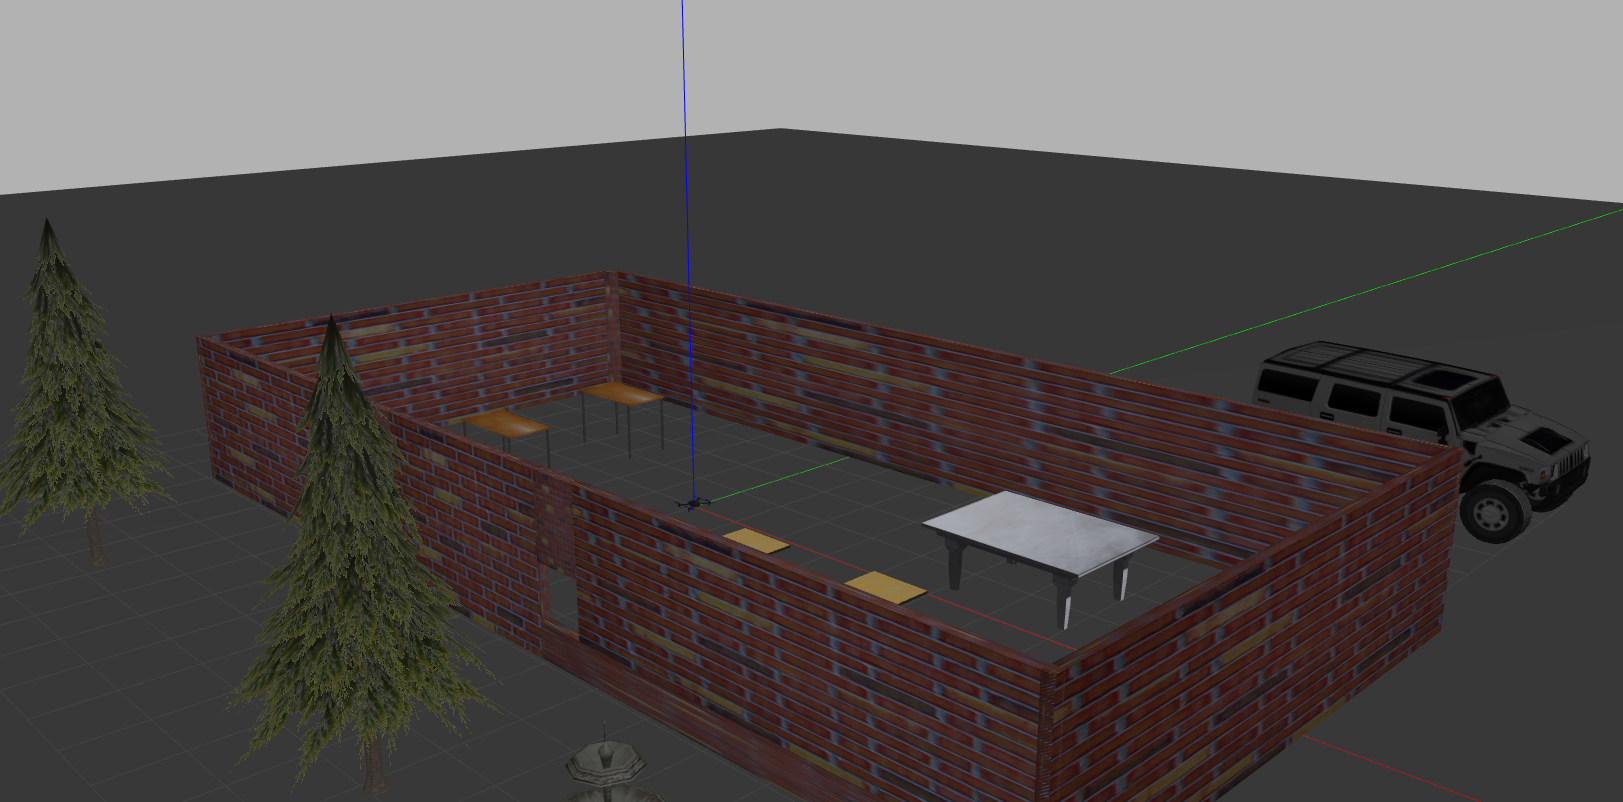
\includegraphics[width=0.7\textwidth]{scene.png}
	\caption{gazebo场景示例}
	\label{fig4-1}
\end{figure}

进入gazebo界面后,使用Control+B进入其编辑界面;之后有两种选择:

\begin{enumerate}
	\item 建立基础模型,一般在这里会绘制上地面及其纹理;如果是室内场景,还会绘制一个大致的墙壁结构,墙壁的纹理,其上的门窗等;最后将该模型保存到.gazebo/model文件中,这是gazebo模型的默认文件。
	\item 直接选择插入模型;可以在此直接插入上文建立的基础模型,也可以插入其他模型库已有的模型,默认存储在/.gazebo/models文件夹下
\end{enumerate}

最后需要将自建场景存储为一个.world文件,gazebo不会给文件后缀的提示,需要自己输入后缀,这一点需要特别注意。在此之后,就获得了自建的world场景,下一步需要在launch文件中更改该项,完成调用。


\subsection{launch文件} \label{4.1.2}

\ref{2.1.2}节中,曾简单介绍launch文件的功能。作为整个仿真环境的配置文件,launch文件中基本包含了仿真所需的参数。

launch文件使用XML标签语言书写,主要为确定启动的节点和加载参数使用,简单的开始节点、加载参数的方法如下:

\begin{minted}[fontsize=\small]{xml}
<node pkg="your package name" name="your node name" type="your node type"/>
<param name="param name" value="param value"/>
<arg name="arg name" default="arg value"/>
\end{minted}

在一个简单的launch文件中,主要会包括设备的信息设置、PX4配置和gazebo仿真配置。

\begin{enumerate}
	\item 设备的信息设置;这一部分包括设备的位姿,通过$x,y,z,R,P,Y$6个变量表示三维位置坐标和滚转、俯仰、偏航姿态角;还包括设置设备的类型和名称,在四旋翼无人机仿真中使用iris作为参数vehicle的值,并且在sdf参数中,将sdf参数的值指向iris的sdf文件(一般在该位置,都使用默认参数加find指令去寻找软件在环仿真的gazebo模型路径);最后是一些gui等参数的设置,默认使用官方设置的即可。
	\item PX4软件在环仿真的参数;在这里启动了名为sitl的节点,其参数指向了EKF设置的rcS文件;
	\item gazebo仿真参数配置;在这里需要修改world\_name参数,其默认是world参数的值,所以实际上也可以直接修改world参数值,将其指向自建的world文件。
\end{enumerate}

自此,launch文件配置完成,可以使用PX4启动launch文件来进行简单的仿真。


\section{单机SLAM仿真}

在进行多机仿真前,首先要进行单机的SLAM仿真,为多机仿真做铺垫。单机SLAM仿真分为单机Offboard模式起降和航路点飞行,以及SLAM下的起降和航路点飞行四步。

\subsection{launch文件配置} \label{4.2.1}

\ref{4.1.2}节中介绍了launch文件的详细配置方法,对于单机的SLAM仿真,配置方法基本与其相同,但是需要给iris无人机加装上双目相机。以下介绍给无人机加装相机的方法:

选择mavros\_posix\_sitl.launch文件,找到设备模型和世界配置区块,原始设置如下:

\begin{minted}[fontsize=\small]{xml}
<!-- vehicle model and world -->
<arg name="est" default="ekf2"/>
<arg name="vehicle" default="iris"/>
<arg name="world" default="$(find mavlink_sitl_gazebo)/worlds/empty.world"/>
<arg name="sdf" default="$(find mavlink_sitl_gazebo)/models/$(arg vehicle)
          /$(arg vehicle).sdf"/>
\end{minted}

加载双目相机,也就是给iris无人机装上相机,需要在设备配置处,加上其附加配置的sdf文件;由于在这里只添加了相机的sdf文件,所以该附加sdf文件不需要手动修改,直接链接到相机上即可。因此需要新建camera参数,其值为iris\_stereo\_camera,是gazebo自带的可以添加到iris无人机上的双目相机,修改后的launch文件部分如下:

\begin{minted}[fontsize=\small]{xml}
<!-- vehicle model and world -->
<arg name="est" default="ekf2"/>
<arg name="vehicle" default="iris"/>
<!-- add stereo camera for iris -->
<arg name="my_camera" default="iris_stereo_camera"/>
<arg name="world" default="$(find mavlink_sitl_gazebo)/worlds
        /empty.world"/>
<!-- also need to revise sdf -->
<arg name="sdf" default="$(find mavlink_sitl_gazebo)/models
        /$(arg my_camera)/$(arg my_camera).sdf"/>
<!-- <arg name="sdf" default="$(find mavlink_sitl_gazebo)/models
        /$(arg vehicle)/$(arg vehicle).sdf"/> -->
\end{minted}

更改完launch文件的无人机配置后,可以试运行来检测,即roslaunch该launch文件。之后有两种方法可以检查,一是使用rostopic list命令,查找当前活跃的话题,如果MAVROS能顺利连接上双目相机,则会出现image\_raw话题(对于双目分为左右,但对于单目仅有一个话题),这种情况下一般是成功的;另一种方法是使用ROS自带的rqt\_graph命令,该命令可以以图的形式展示出,这种方式用途更广。装配成功后,仿真加载时应如图\ref{fig4-2}所示:

% 或许可以加一张大图

\begin{figure}[!ht]
	\centering
	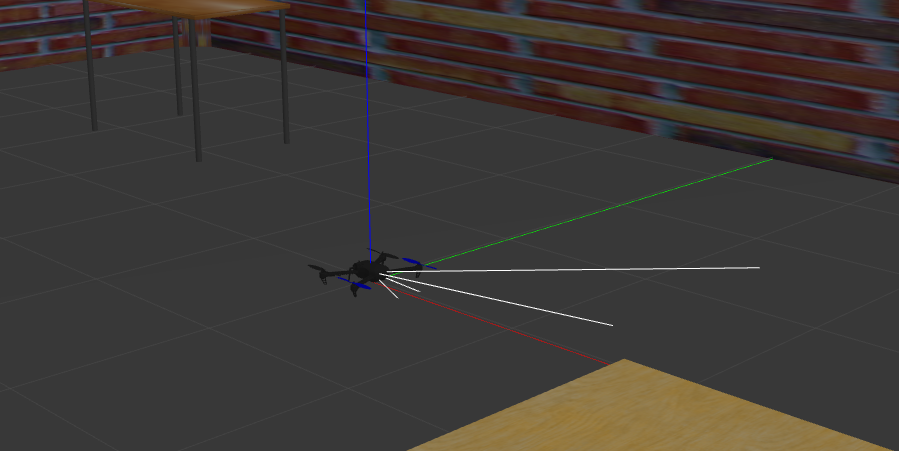
\includegraphics[width=0.7\textwidth]{mono_uav.png}
	\caption{装配相机的iris无人机}
	\label{fig4-2}
\end{figure}

需要注意,在需要与MAVROS建立通信的launch文件中,需要设置fcu端口号,具体表示为udp+本地端口号,在多机的launch文件中,每一架飞机的端口号都是不同的,但单机不需要作出修改。

如果设置双目相机参数后加载失败或加载到一个正方体模型,则是双目相机模型缺失导致的。一种方法是删除gazebo自带的models中的双目相机,并用PX4中的双目相机飞机代替;另一种方法则是直接将sdf的值指向PX4的双目相机飞机,即其值为PX4双目相机飞机的路径。

\subsection{Offboard程序} \label{4.2.2}

完成双目相机的配置后,第二步是进入Offboard程序。与\ref{2.2.3}的Offboard模式类似,首先目标是完成一套完整的起飞降落。需要注意,Offboard模式中,所有消息指令都需要以大于$2Hz$的频率发送,否则会激活安全生效机制,飞机返航。

\begin{enumerate}
	\item 起飞的方式。动力学模型上的起飞即给四旋翼增加动力,保持平衡并提供向上的大于重力的升力,在程序中表示为发布位置指令,该消息类型为MAVROS的geometry\_msgs数据类型。
	\item 降落的方式。一般使用切换飞行模式的方法,将飞行模式切换到降落模式,选择降落模式中的自动降落即可。
\end{enumerate}

降落的程序如下:

\begin{minted}[fontsize=\small]{cpp}
// proceed landing process
ROS_INFO("landing");
mavros_msgs::SetMode land_set_mode;
land_set_mode.request.custom_mode = "AUTO.LAND";
while (ros::ok()){
    if( current_state.mode != "AUTO.LAND" &&
        (ros::Time::now() - last_request > ros::Duration(5.0))){
        if( set_mode_client.call(land_set_mode) &&
            land_set_mode.response.mode_sent){
            ROS_INFO("Land enabled");
        }
        last_request = ros::Time::now();
    }
    if(!current_state.armed){
        break;
    }

    ros::spinOnce();
    rate.sleep();
}
\end{minted}

航路点飞行的简单实现方法为,依次发布各航路点的位置信息,但需要一个函数去判断飞机是否到达了航路点。函数的实现可以利用预计坐标和现处位置之间的欧式距离作评判标准,小于某值则认为到达航路点,实现的关键在现处位置消息的订阅。首先需要定义current\_pose作为现处位置的变量,之后定义回调函数,获得该信息,实现的代码如下:

\begin{minted}[fontsize=\small]{cpp}
// record current pose
geometry_msgs::PoseStamped current_pose; /* NOLINT */

// callback function for Subscriber for local_pos_sub
void local_cb(const geometry_msgs::PoseStamped::ConstPtr& msg){
    current_pose = *msg;
}
\end{minted}

检查是否到达航路点的函数如下:

\begin{minted}[fontsize=\small]{cpp}
// check if reached a waypoint
bool check_waypoint(const geometry_msgs::PoseStamped &now_pose, 
    const geometry_msgs::PoseStamped &aim_pose){
    // define Point to hold current position and aim position
    geometry_msgs::Point curr, aim;
    curr = now_pose.pose.position;
    aim = aim_pose.pose.position;
    double precision = 0.1;

    // define return value
    bool reach = false;

    // calculate distance
    double dist = sqrt(pow((curr.x - aim.x), 2) +
    pow((curr.y - aim.y), 2) + pow((curr.z - aim.z), 2));
    if(dist < precision){
        reach = true;
        ROS_INFO("reached waypoint!");
    }

    return reach;
}
\end{minted}

前往下一个航路点的方法如下:

\begin{minted}[fontsize=\small]{cpp}
// set second waypoint
geometry_msgs::PoseStamped pose2;
pose2.pose.position.x = 2;
pose2.pose.position.y = 2;
pose2.pose.position.z = 2;

// heading for waypoint 2
while(ros::ok()){
    // publish pose1 information
    local_pos_pub.publish(pose2);
    ros::spinOnce();

    // check if reached a waypoint
    if (check_waypoint(current_pose, pose2)) break;
    rate.sleep();
}
\end{minted}

按2个航路点飞行的地面站轨迹示意图如图\ref{fig4-3}所示:

\begin{figure}[!ht]
	\centering
	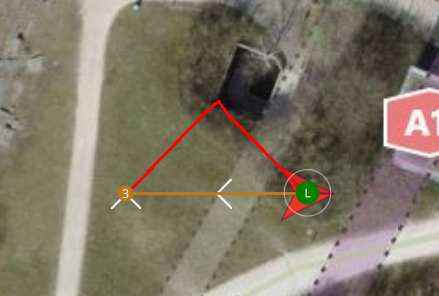
\includegraphics[width=0.6\textwidth]{waypoint.png}
	\caption{地面站的航路点飞行轨迹}
	\label{fig4-3}
\end{figure}

\subsection{视觉定位的坐标变换} \label{4.2.3}

在正常GPS定位的Offboard模式下,飞机的位置在MAVROS中作为已知量存在。但在视觉定位模式下,可以参照图\ref{fig4-5}的节点与话题关系,MAVROS需要通过vision\_pose/pose话题获得飞机的位姿信息。而ORB-SLAM2解算出的位姿并不是MAVROS的地理位置消息格式,因此需要做一些转换。

%\begin{figure}[!ht]
%	\centering
%	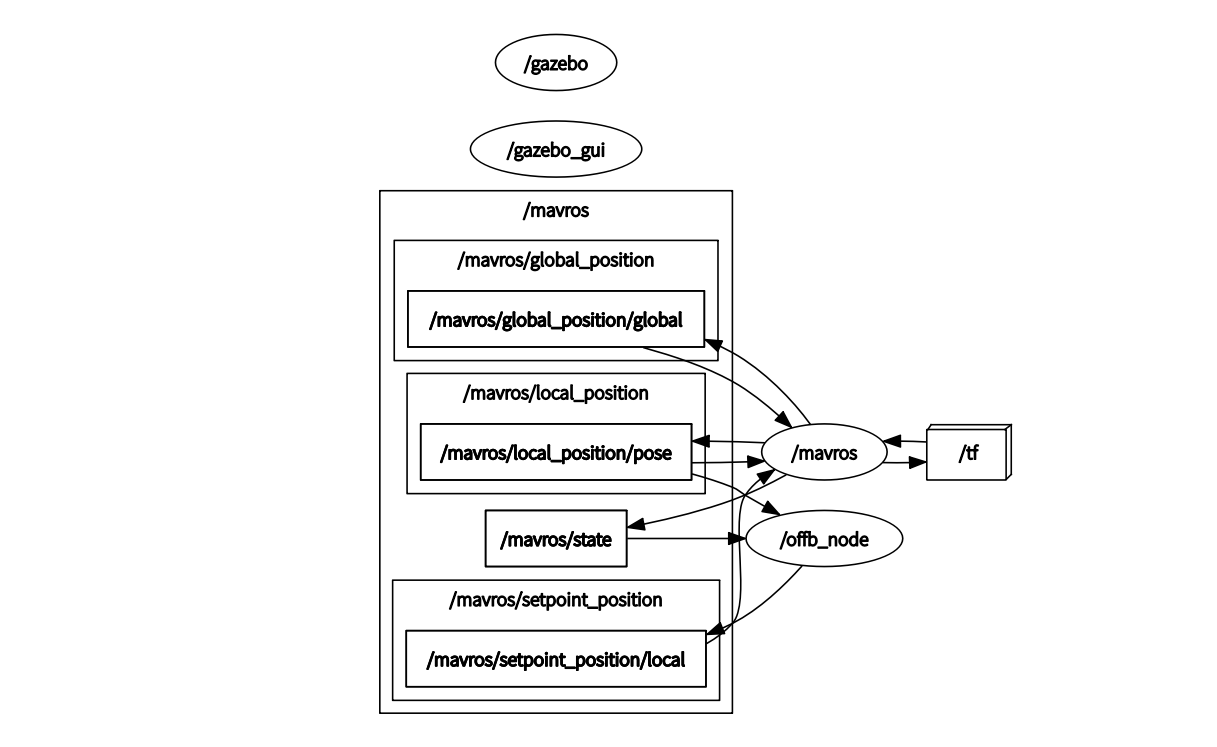
\includegraphics[width=0.8\textwidth]{rqtOffboard.png}
%	\caption{Offboard节点话题关系}
%	\label{fig4-4}
%\end{figure}

\begin{figure}[!ht]
	\centering
	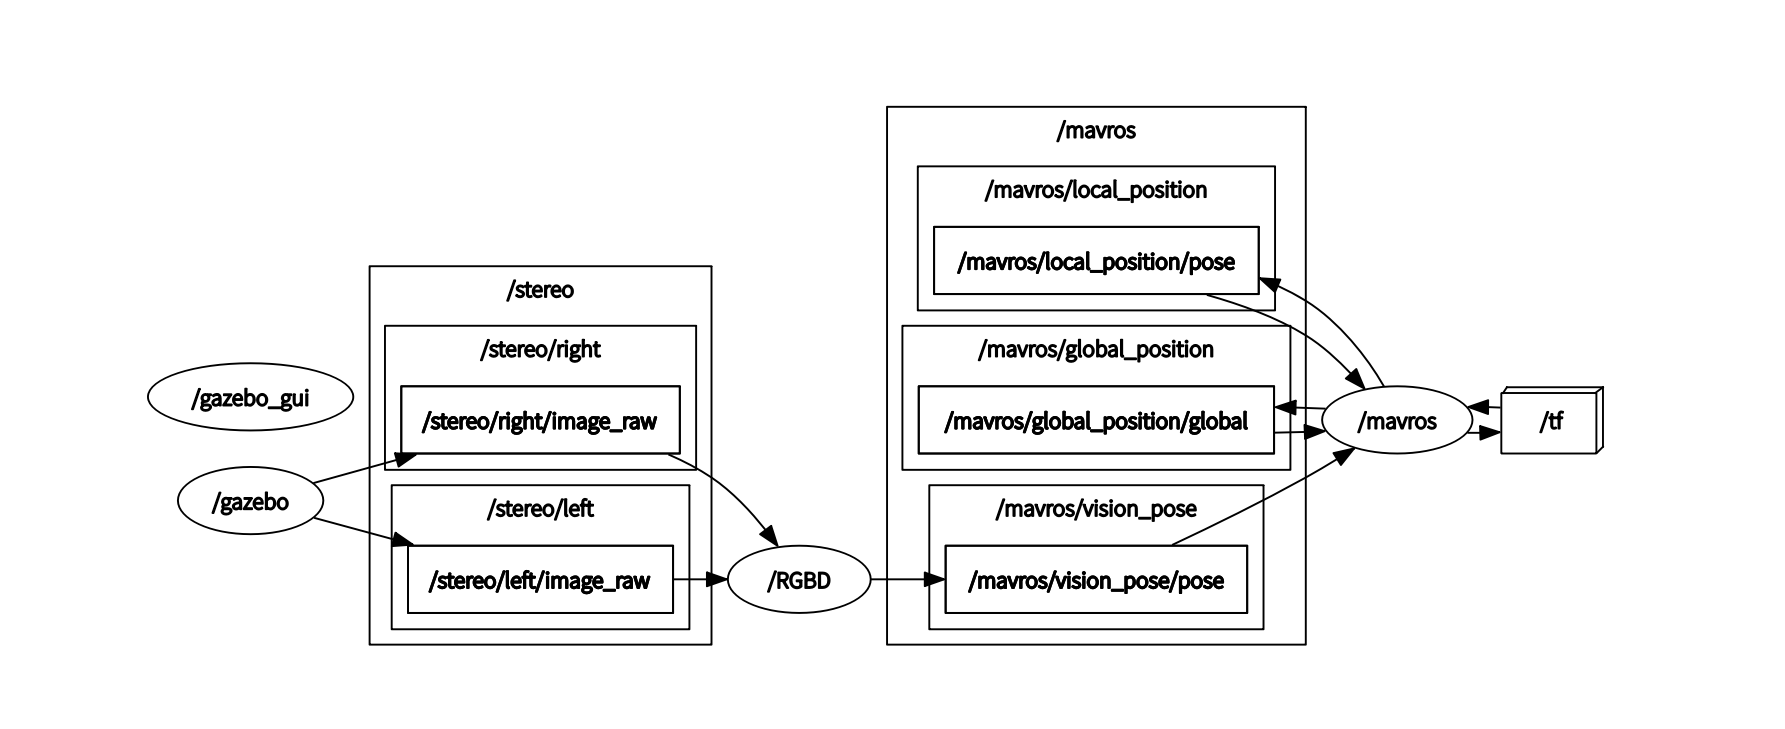
\includegraphics[scale=0.25]{rqtRGBD.png}
	\caption{视觉SLAM节点话题关系}
	\label{fig4-5}
\end{figure}

ORB-SLAM2得到的外参$\bf{Tcw}$矩阵为$4 \times 4$矩阵:

\begin{equation}
\bf{Tcw}=\begin{bmatrix}
\bf{R_{cw}} & \bf{t_{cw}}\\0 & 1
\end{bmatrix}
\end{equation}

其中,$\bf{R_{cw}}$为旋转矩阵,$\bf{t_{cw}}$为平移向量。

可以证明,从相机的外参矩阵得到相机位姿:

\begin{equation}
\begin{aligned}
\bf{R_{wc}}= &\bf{R_{cw}}^T\\
\bf{t_{wc}}= &-\bf{R_{wc}} \cdot  \bf{t_{cw}}
\end{aligned}
\end{equation}

在此之后,还需要将$\bf{R_{wc}}$和$\bf{t_{wc}}$赋值给ROS中tf坐标系类型的Transform变量,之后通过调用ROS的poseTFToMsg函数,将tf类型的变量转为MAVROS的地理位置消息类型变量。实现的代码如下:

\begin{minted}[fontsize=\small]{cpp}
Rwc = Tcw.rowRange(0,3).colRange(0,3).t(); // Rotation information
twc = -Rwc*Tcw.rowRange(0,3).col(3); // translation information
vector<float> q = ORB_SLAM2::Converter::toQuaternion(Rwc);

tf::Transform new_transform;
new_transform.setOrigin(tf::Vector3(twc.at<float>(0, 0), 
twc.at<float>(0, 1), twc.at<float>(0, 2)));

tf::Quaternion quaternion(q[0], q[1], q[2], q[3]);
new_transform.setRotation(quaternion);

tf::poseTFToMsg(new_transform, pose.pose);
x = pose.pose.position.x;
y = pose.pose.position.y;
z = pose.pose.position.z;
pose.pose.position.x = z;
pose.pose.position.y = -x;
pose.pose.position.z = -y;
pose_pub->publish(pose);
\end{minted}

\subsection{MAVROS键盘控制} \label{4.2.4}

尽管可以使用Offboard模式下的position信息进行航路点的控制,但是无人机起飞和前进的动作幅度过大,直接影响了SLAM系统的跟踪效果,因此需要考虑通过MAVROS发布的信息,对无人机的速度进行详细控制。

可以选择设置其速度,利用循环控制话题执行的时间来设置距离的方法,但该方法在灵活性上有所欠缺;为了更加真实地进行无人机的仿真,本文研究了一套利用键盘输入信息控制无人机飞行的程序。

首先,在对MAVROS的话题进行分析后,发现其订阅的话题有setpoint\_velocity下的cmd\_vel\_unstamped话题;该话题用于发送速度信息给FCU处理,因此本程序的核心为手动控制发送给FCU的速度信息,即MAVROS订阅的速度信息。

该信息属于地理信息的Twist类型,该类型包含三方向的线速度和角速度,因此可以通过更改信息的内容并且完成发布,则MAVROS会订阅并接收到该消息,完成对其速度的控制。

以键盘上的T和W为例,两者分别代表进行切换模式起飞与增加X方向的速度:

\begin{minted}[fontsize=\small]{cpp}
    case KEYCODE_T:
        ROS_INFO("Command Offboard mode RECEIVED!");
        Offboard(set_mode_client, offb_set_mode, arm_cmd,
            arming_client, local_pos_pub, pose, rate);
        velocityTuning(twist, 0);
        flag = true;
        break;
    case KEYCODE_W:
        ROS_INFO("Command Add forward speed RECEIVED!");
        velocityTuning(twist, 1);
        flag = true;
        break;
\end{minted}

在这之中用到了自定义的velocityTuning函数,其作用是根据第二个参数的值完成对应线速度或角速度的预设变化。其中的标志位flag用来给switch语句结束后判断是否应该发送twist的速度信息,并且在发送过后重新将标志位设为false。

\subsection{单机仿真实验结果} \label{4.2.5}

首先尝试了在简单的gazebo环境中进行起飞,场景如图\ref{fig4-6-1}所示;由于使用双目相机,不需要初始化过程,因此飞机在非速度控制下的起飞中,也能匹配到较多特征点,但由于轨迹较短,并不能展示出完成的稀疏地图。

\begin{figure}[htbp]
	\centering
	\begin{minipage}[t]{0.45\columnwidth} %小于1/n如果使用n张图片
		\centering
		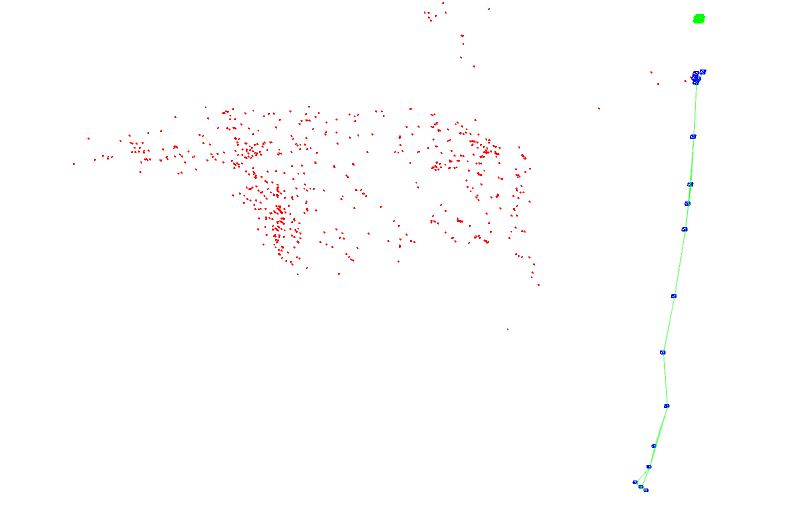
\includegraphics[width=1.0\columnwidth]{single.png}
		\caption{起飞过程的轨迹与建图}
		\label{fig4-6}
	\end{minipage}
	\begin{minipage}[t]{0.45\columnwidth}
		\centering
		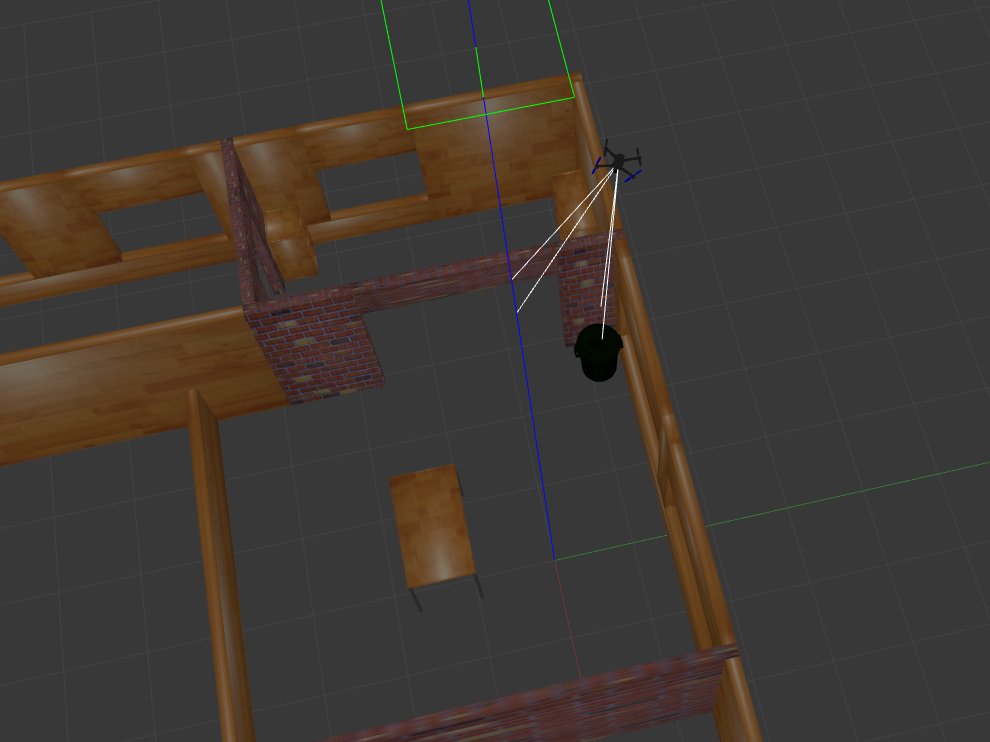
\includegraphics[width=1.0\columnwidth]{single1.png}
		\caption{起飞过程的场景}
		\label{fig4-6-1}
	\end{minipage}
\end{figure}

在这之后,使用图\ref{4.2.4}中设计的键盘控制程序,更换了比较复杂的场景进行仿真,图\ref{fig4-6-2}为场景的俯视图,处在一个类似迷宫的墙壁之中,沿墙壁边缘行进,并在行进过程中不断转动视角以探测自身周边的特征点;其结果如图\ref{fig4-6-3},\ref{fig4-6-4},\ref{fig4-6-5}所示,最终逐渐构建出了半个地图场景的轮廓。

\begin{figure}[htbp]
	\centering
	\begin{minipage}[t]{0.24\columnwidth} %小于1/n如果使用n张图片
		\centering
		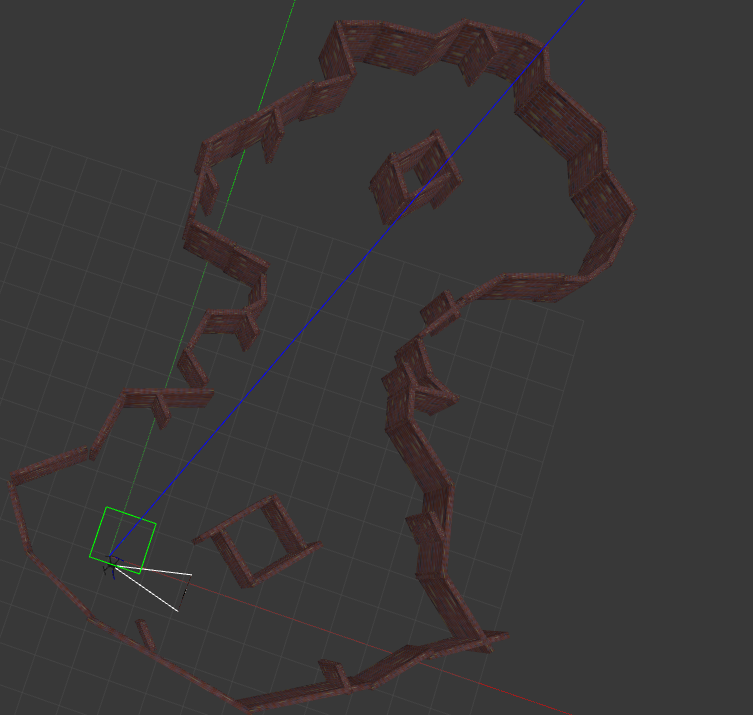
\includegraphics[width=1.0\columnwidth]{single2.png}
		\caption{场景俯视图}
		\label{fig4-6-2}
	\end{minipage}
	\begin{minipage}[t]{0.24\columnwidth}
		\centering
		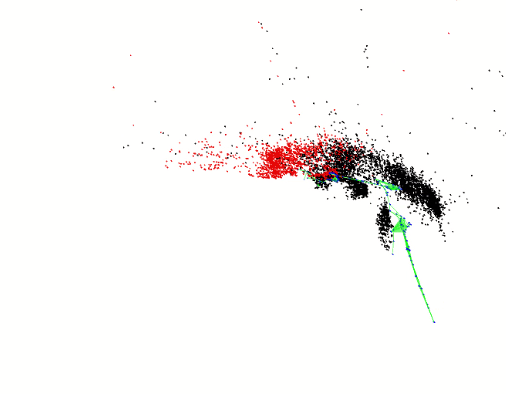
\includegraphics[width=1.0\columnwidth]{single3.png}
		\caption{阶段1}
		\label{fig4-6-3}
	\end{minipage}
	\begin{minipage}[t]{0.24\columnwidth}
		\centering
		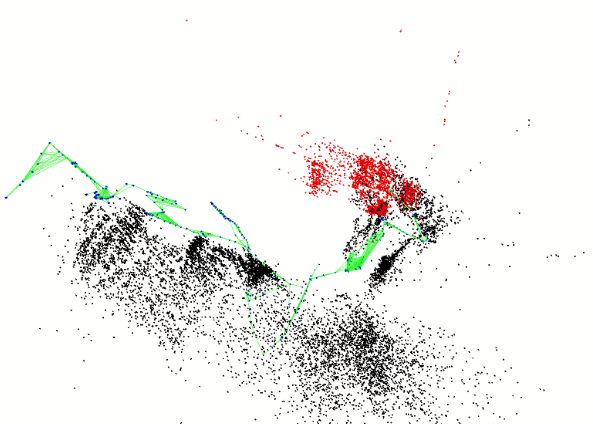
\includegraphics[width=1.0\columnwidth]{single4.png}
		\caption{阶段2}
		\label{fig4-6-4}
	\end{minipage}
	\begin{minipage}[t]{0.24\columnwidth}
		\centering
		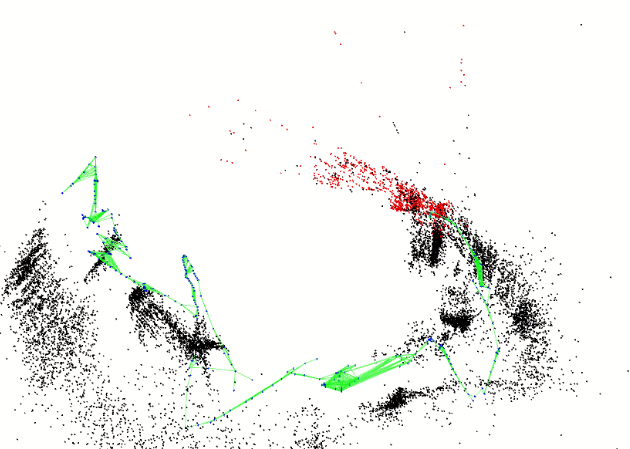
\includegraphics[width=1.0\columnwidth]{single5.png}
		\caption{阶段3}
		\label{fig4-6-5}
	\end{minipage}
\end{figure}


\section{多机SLAM仿真}

进行多机仿真是本文的核心内容,但由于计算机硬件的限制,无法在gazebo环境中做到真正的集群。因此本文采用三架iris无人机进行多机编队与航路点飞行的仿真,采用两架携带单目相机的iris进行双机协同SLAM仿真。

\subsection{launch文件配置} \label{4.3.1}

多机配置与单机配置最大的区别是,引用的子文件不同;单机引用posix\_sitl文件,而多机则引用vehicle\_spawn文件,而spawn文件是多机所独有的。

进入多机的launch文件,则需要引入组的概念。一个组使用一个命名空间,具有一套MAVROS的配置信息,多个组可以并行存在。因此在多机的launch文件设计中,一个组就是一架飞机,需要设置该组的命名空间,该组下的所有话题将共同使用该命名空间开头的话题。除此之外,还需要修改无人机的ID,ID默认从0到10;之后修改fcu地址和MAVLINK的udp端口,一般在末尾加上该无人机的ID即可。完整的双机launch配置代码如下:

\begin{minted}[fontsize=\small]{xml}
<!-- UAV0 -->
<group ns="uav0">
<!-- MAVROS and vehicle configs -->
<arg name="ID" value="0"/>
<arg name="fcu_url" default="udp://:14540@localhost:14580"/>
<!-- PX4 SITL and vehicle spawn -->
<include file="$(find px4)/launch/single_vehicle_spawn_rcs.launch">
    <arg name="x" value="0"/>
    <arg name="y" value="0"/>
    <arg name="z" value="0"/>
    <arg name="R" value="0"/>
    <arg name="P" value="0"/>
    <arg name="Y" value="0"/>
    <arg name="vehicle" value="$(arg vehicle)"/>

    <arg name="my_camera" value="iris_fpv_cam"/>

    <arg name="mavlink_udp_port" value="14560"/>
    <arg name="mavlink_tcp_port" value="4560"/>
    <arg name="ID" value="$(arg ID)"/>
    <arg name="gst_udp_port" value="$(eval 5600 + arg('ID'))"/>
    <arg name="video_uri" value="$(eval 5600 + arg('ID'))"/>
    <arg name="mavlink_cam_udp_port" value="$(eval 14530 + arg('ID'))"/>

</include>
<!-- MAVROS -->
<include file="$(find mavros)/launch/px4.launch">
    <arg name="fcu_url" value="$(arg fcu_url)"/>
    <arg name="gcs_url" value=""/>
    <arg name="tgt_system" value="$(eval 1 + arg('ID'))"/>
    <arg name="tgt_component" value="1"/>
</include>
</group>
\end{minted}

其默认每架无人机调用的是spawn文件,其中关键的模型组合有两种方式,一种是使用urdf进行模型配置,一种是使用新的sdf。具体使用哪种视PX4的版本而定,由于urdf模型的配制方法要旧于sdf,新版的PX4统一使用sdf进行gazebo仿真的模型配置,并且使用jinja.py脚本生成sdf模型配置。

\begin{figure}[!ht]
	\centering
	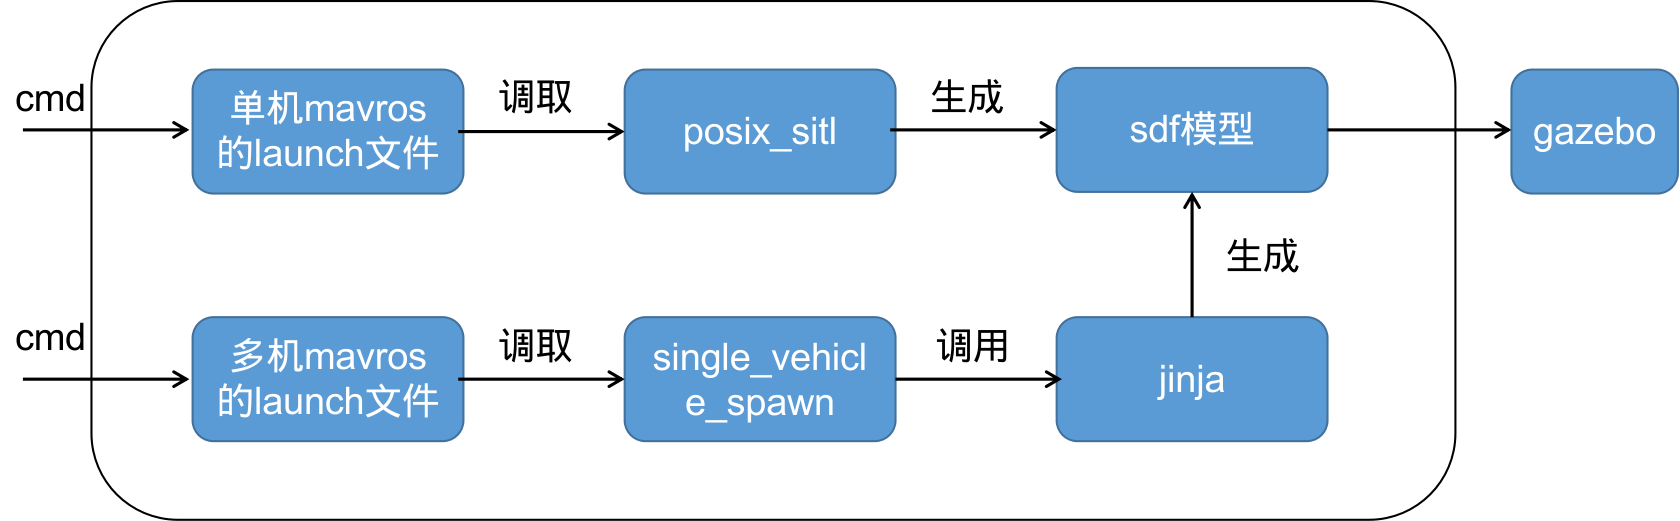
\includegraphics[width=0.9\textwidth]{sdf.png}
	\caption{仿真模型生成流程}
	\label{fig-sdf}
\end{figure}

图\ref{fig-sdf}展示了PX4中使用gazebo生成模型的方法,决定了修改模型的方法。可以看出,launch文件分为顶层和底层文件;平常直接使用roslaunch命令启动的一般为顶层文件,而顶层文件中调取的一般为底层文件。对于单机和多机,其调用的底层文件不同;单机调取posix\_sitl.launch文件,而多机则调取single\_vehicle\_spawn文件。二者的区别是单机的底层文件直接使用了即有的sdf模型,但多机的底层文件基于spawn繁殖机制,重新调用jinja生成了新的sdf模型,并且在该过程中对MAVLINK的许多参数作了配置,这一点是单机所没有的。最终都生成gazebo可以加载出的模型文件。

旧版本使用urdf版本的PX4,如果在launch文件中直接将其修改为sdf格式生成的模型,一般会报错jinja.py文件中有很多参数未定义,一种简单的处理方式是直接将新版本的janja替换到旧版本中去(为什么要使用旧版本,因为新版本的稳定性可能存在一些问题),但是这样做可能会连带产生一些附加问题,尽量选择不修改jinja这种较为底层的文件。

由于ROS的机制,话题如果重复,则会报错,并用时间戳最新的话题替换掉时间戳更旧的话题;如果多架无人机的话题不加以区分,可能会导致最终话题重复,从而只有一架无人机可以使用。


\subsection{多机编队控制} \label{4.3.2}

多机的控制可以使用编队控制,控制方法可以分为两种:集中式和分布式。

\begin{enumerate}
	\item 集中式即集群中存在领机,其他飞机需要跟随领机的运动轨迹。这种方式的实现相对简单,需要各机实时订阅领机的位置,并且始终和领机保持设定好的队形,也就是相对位置。
	\item 分布式则没有领机的概念,各无人机按照各自设定好的航路点行进,该方式的实现方法主要需要依靠多线程的设计。
\end{enumerate}

当无人机数量较多时,可以采用分级跟随的办法,假设有N架无人机,则构建一个$N \times N$邻接矩阵$T$,这里以$N=5$为例:

$$
T=\begin{bmatrix}
0 & 0 & 0 & 0 & 0\\
1 & 0 & 0 & 0 & 0\\
1 & 1 & 0 & 0 & 0\\
0 & 1 & 1 & 0 & 0\\
0 & 0 & 1 & 1 & 0
\end{bmatrix}
$$

若$N_{i,j}>0$,则$i,j$之间会建立通信,如图\ref{fig4-7}所示:

\begin{figure}[!ht]
	\centering
	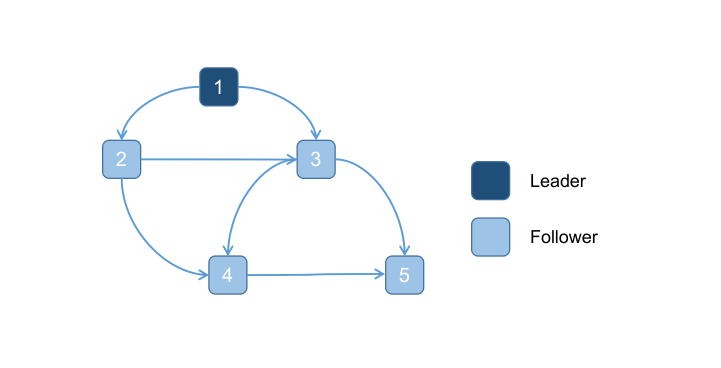
\includegraphics[width=0.6\textwidth]{formation.png}
	\caption{编队通信方法}
	\label{fig4-7}
\end{figure}

有$N_{2,1},N_{3,1},N_{3,2},N_{4,2},N_{4,3},N_{5,3},N_{5,4}$均不为0,则在这些对之间,按由小到大的顺序建立通信,传输长机的位置信息,保持相对位置的跟随。

在无人机发生编队队形变换时,则需要考虑最小总路径,可以用KM匈牙利算法解得每一架飞机对应的最小路径,并且在队形变换过程中需要考虑碰撞的影响\cite{XiaoKun}。

图\ref{fig4-8}展示了三机编队的仿真结果,

%\begin{figure}[!ht]
%	\centering
%	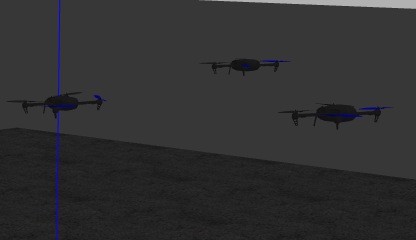
\includegraphics[width=0.5\textwidth]{multi.png}
%	\caption{三机编队仿真}
%	\label{fig4-8}
%\end{figure}


% 注意caption (a)(b)
\begin{figure}[htbp]
	\centering
	\begin{minipage}[t]{0.45\columnwidth} %小于1/n如果使用n张图片
		\centering
		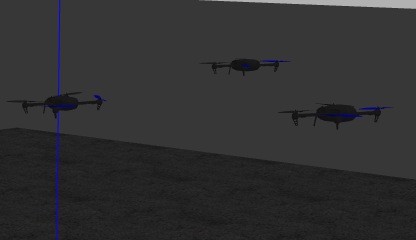
\includegraphics[width=1.0\columnwidth]{multi.png}
		\caption{三机编队仿真}
		\label{fig4-8}
	\end{minipage}
	\begin{minipage}[t]{0.45\columnwidth}
		\centering
		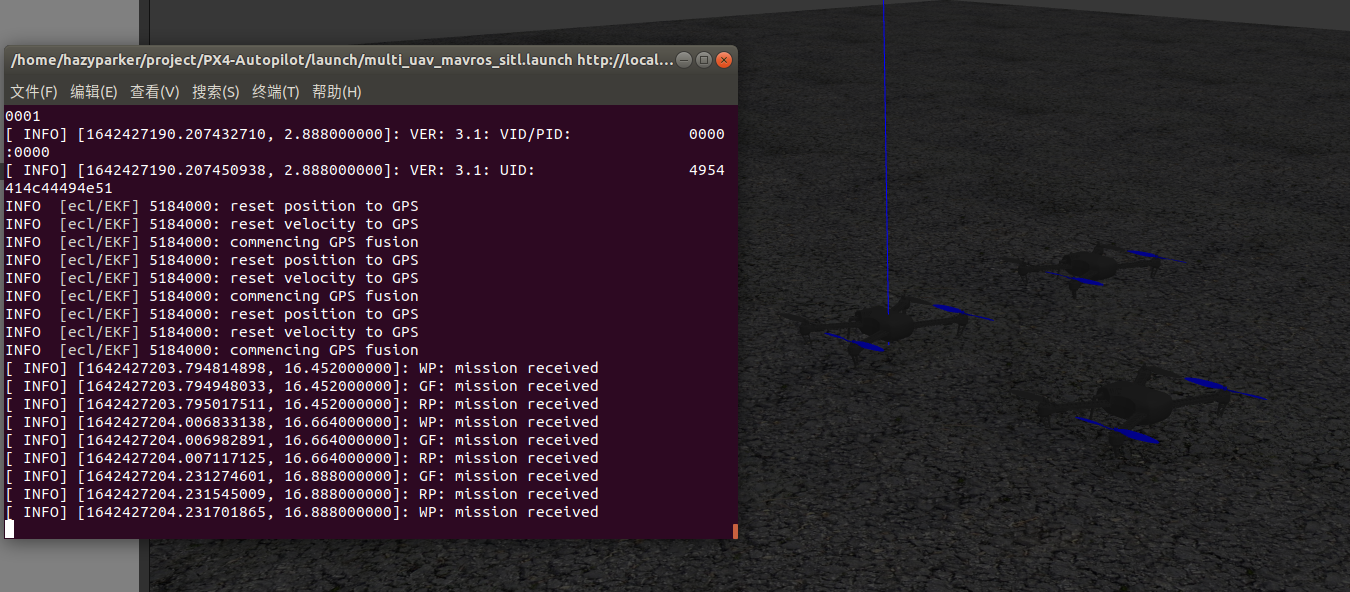
\includegraphics[width=1.0\columnwidth]{multi1.png}
		\caption{三机跟随仿真}
		\label{fig4-8-1}
	\end{minipage}
\end{figure}


\subsection{多机SLAM仿真} \label{4.3.3}

多机SLAM仿真除PX4的配置外,还要对SLAM的launch文件进行配置。其中包含了设置相机的参数文件,更重要的是配置各无人机所接受的相机话题。

\begin{figure}[!ht]
	\centering
	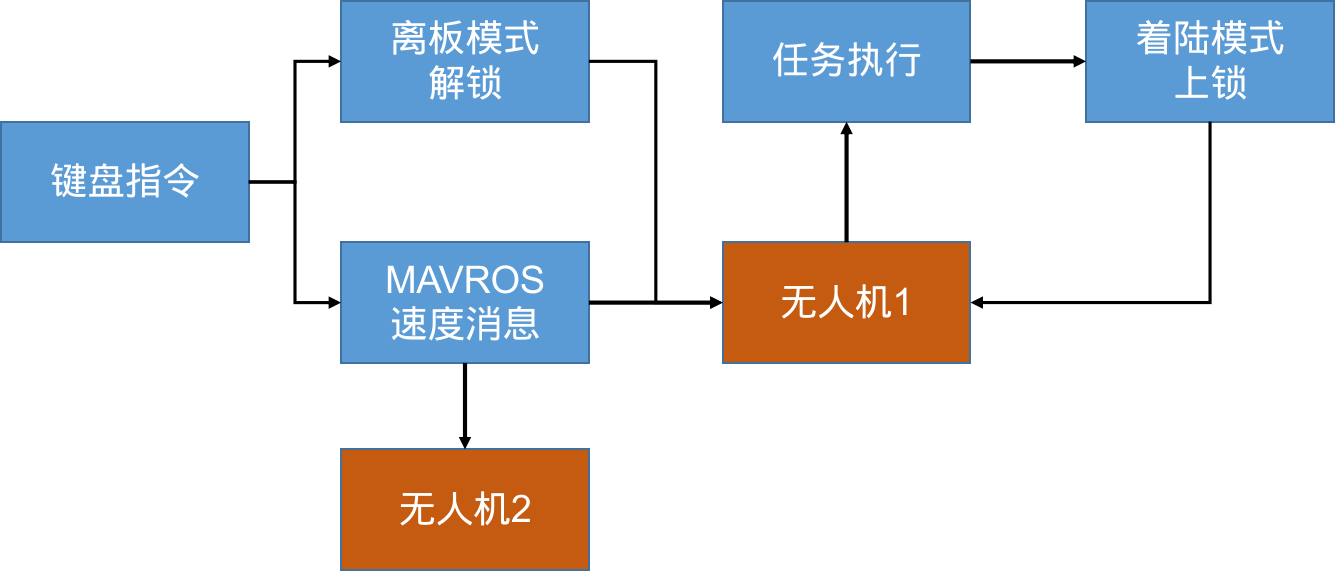
\includegraphics[width=0.7\textwidth]{multi3.png}
	\caption{双机控制策略}
	\label{fig-multicontrol}
\end{figure}

考虑到仿真环境中场景比较复杂,容易发生碰撞,本文的多机协同SLAM仿真并没有采取多机编队仿真的方式,而是仿照CCM-SLAM真机实验的方式,采取了“手飞”,即键盘控制下的仿真飞行。

考虑到键盘按键有限,因此不采用一个键盘分别控制两架无人机的方式,而是利用了PX4解锁的机制,分别对两架无人机进行切换离板模式和解锁。如图\ref{fig-multicontrol}无人机1与无人机2接收到的速度变化指令是一致的。当无人机1解锁起飞后,无人机2并没有解锁,因此发送的速度指令并不会导致无人机2做出任何响应;直至无人机1完成任务并且返航后,无人机2再根据自己的发布者和订阅者完成切换模式和解锁,此时接收到的MAVROS指令开始对无人机2起作用,其开始正常工作。

启动时需要启动服务器和客户端,然后打开ORB-SLAM节点,最终结果如图:

\begin{figure}[htbp]
	\centering
	\begin{minipage}[t]{0.45\columnwidth} %小于1/n如果使用n张图片
		\centering
		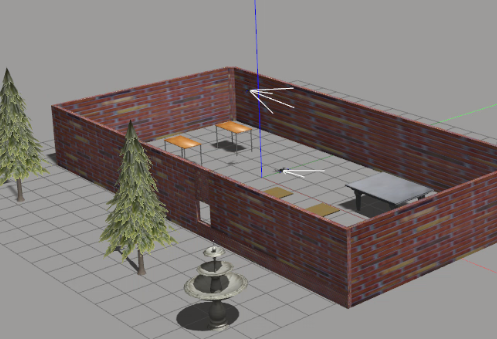
\includegraphics[width=1.0\columnwidth]{ccmsim2.png}
		\caption{仿真场景}
		\label{fig4-9}
	\end{minipage}
	\begin{minipage}[t]{0.45\columnwidth}
		\centering
		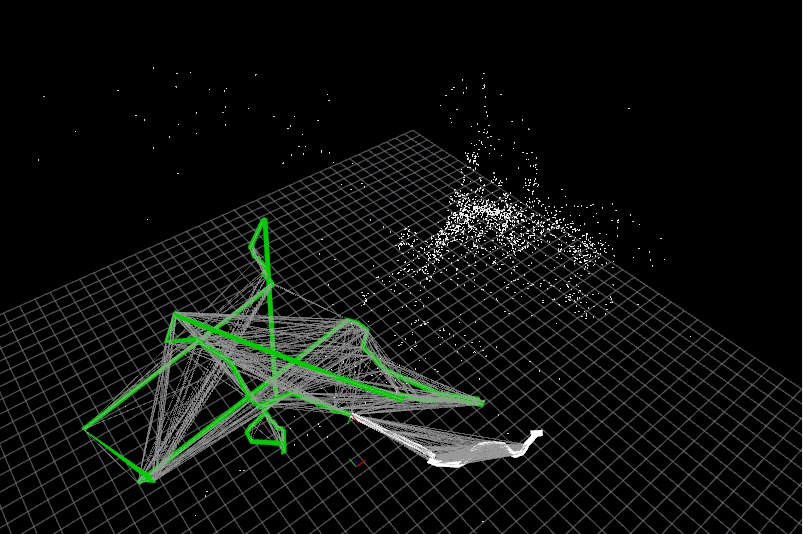
\includegraphics[width=1.0\columnwidth]{ccmsim1.png}
		\caption{建图情况}
		\label{fig4-9-1}
	\end{minipage}
\end{figure}

从两架无人机的位姿轨迹中可以看出,在没有GPS信息传递的情况下,基本凭外观相似到slam的定位完成了两架飞机位姿关系的计算,从而完成了地图拼合。



































